\chapter{Evaluation and Results}
\label{chap:evaluation_results}

Models that achieved the best validation \gls{SSIM} values during the training were analyzed. For the investigation, I used the third distinct dataset. I used full resolution 544×352 images, without cropping, as the factors of the image sides are $544 = 2^5\times 17^1$ and $352 = 2^5\times 11^1$. Therefore the five max-pooling layers with 2×2 kernel and 2×2 will behave the same as in training. I tested the models in evaluation mode and on the same metrics as in the section \ref{subsec:training}. While the models in evaluation mode are not inherently stochastic, they can introduce some level of randomness if there are any numerical instabilities during the computation. I ran ten tests on the dataset to obtain accurate results and calculated the average. Average values over the runs for the UNet were:

\begin{align*}
    &\texttt{\gls{SSIM}}: 0.8784421, & &\texttt{\gls{MAE}}: 0.0126786, & &\texttt{\gls{MSE}}: 0.0021389
\end{align*}

\noindent and for the \gls{GUNet} were:
\begin{align*}
    &\texttt{\gls{SSIM}}: 0.8782260, & &\texttt{\gls{MAE}}: 0.0125654, & &\texttt{\gls{MSE}}:0.0020741.
\end{align*}

\section{Comparison of Forecasts}
\label{sec:comparison}

Both networks generally fail to predict the location of the most intense storms and tend to spread the higher-intensity clusters more and more as the predictions advance. To present the differences in the weather forecasts produced by the models, I created a visualization of the outputs side by side with the observed weather phenomena. I decided to crop all the ground truth observations and network outputs to images with resolution 256×256, as portrayed in figure \ref{fig:comparison_06_cutout}, to better visualize the cloud structure.

\begin{figure}[ht]
    \centering
    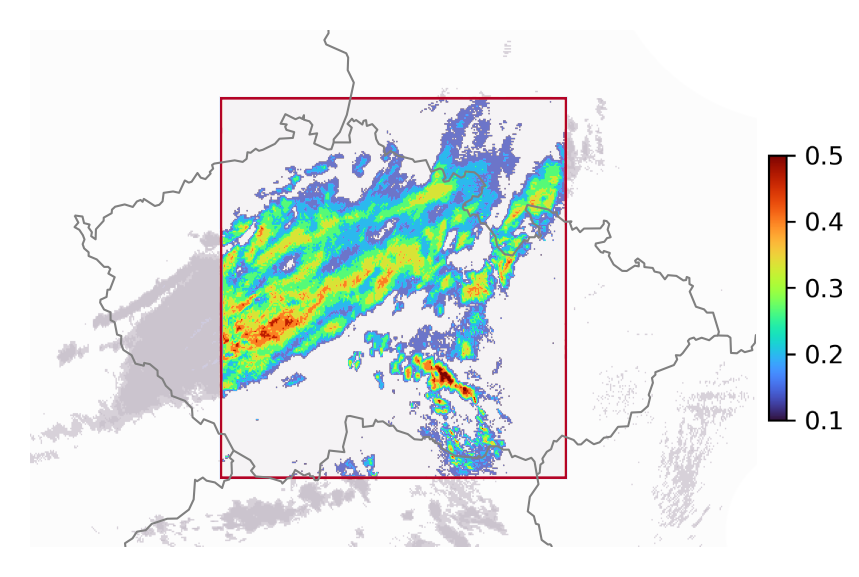
\includegraphics[width=\textwidth]{images/comparison_square_06_cutout.png}
    \caption[Cutout which was used for the comparisons of predictions]{\label{fig:comparison_06_cutout}Cutout which was used for images in figure \ref{fig:comparison_06}.}
\end{figure}

 For further improvements in the visual comparison, I restricted the color bar in the visualization to only show values between lower bound $l$ and upper bound $h$. I adjusted the alpha value of each pixel $x$ in each image to have the value:

\begin{equation}
    \text{f}(x)=\max\left(0,\tanh\left(4\pi\frac{\left(x-l\right)}{h-l}\right)\right).
\end{equation}

 The alpha values guarantee a smooth change to transparency when the pixel's value approaches $l$. If a pixel's value is greater than $h$, it is adjusted to match the value of $h$.

Figure \ref{fig:comparison_06} illustrates the predictions made by \gls{GUNet} and UNet for a particular set of inputs and targets. Only four out of the eight targets and outputs are displayed, while the inputs are not shown. The predictions are spaced 20 minutes apart, enabling more evident observation of cloud movement and future prediction changes. The \gls{SSIM} and \gls{MAE} computed from the cutouts are provided below each prediction.

To see additional examples, please refer to figures \ref{fig:comparison_01}, \ref{fig:comparison_09}, \ref{fig:comparison_07}, and \ref{fig:comparison_04} in appendix \ref{apx:comparisons}. In figure \ref{fig:comparison_01}, you will find a situation with higher-intensity radar echoes, while figure \ref{fig:comparison_09} displays more complex cloud formations on radar images. The other images were chosen from a randomized batch of data points from the test dataset to ensure an unbiased selection. To guarantee that the images included radar echoes, To sort the data points, I utilized the mean value of the pixels in the inputs and then chose the images that had the highest mean values.

\begin{figure}[H]
    \centering
    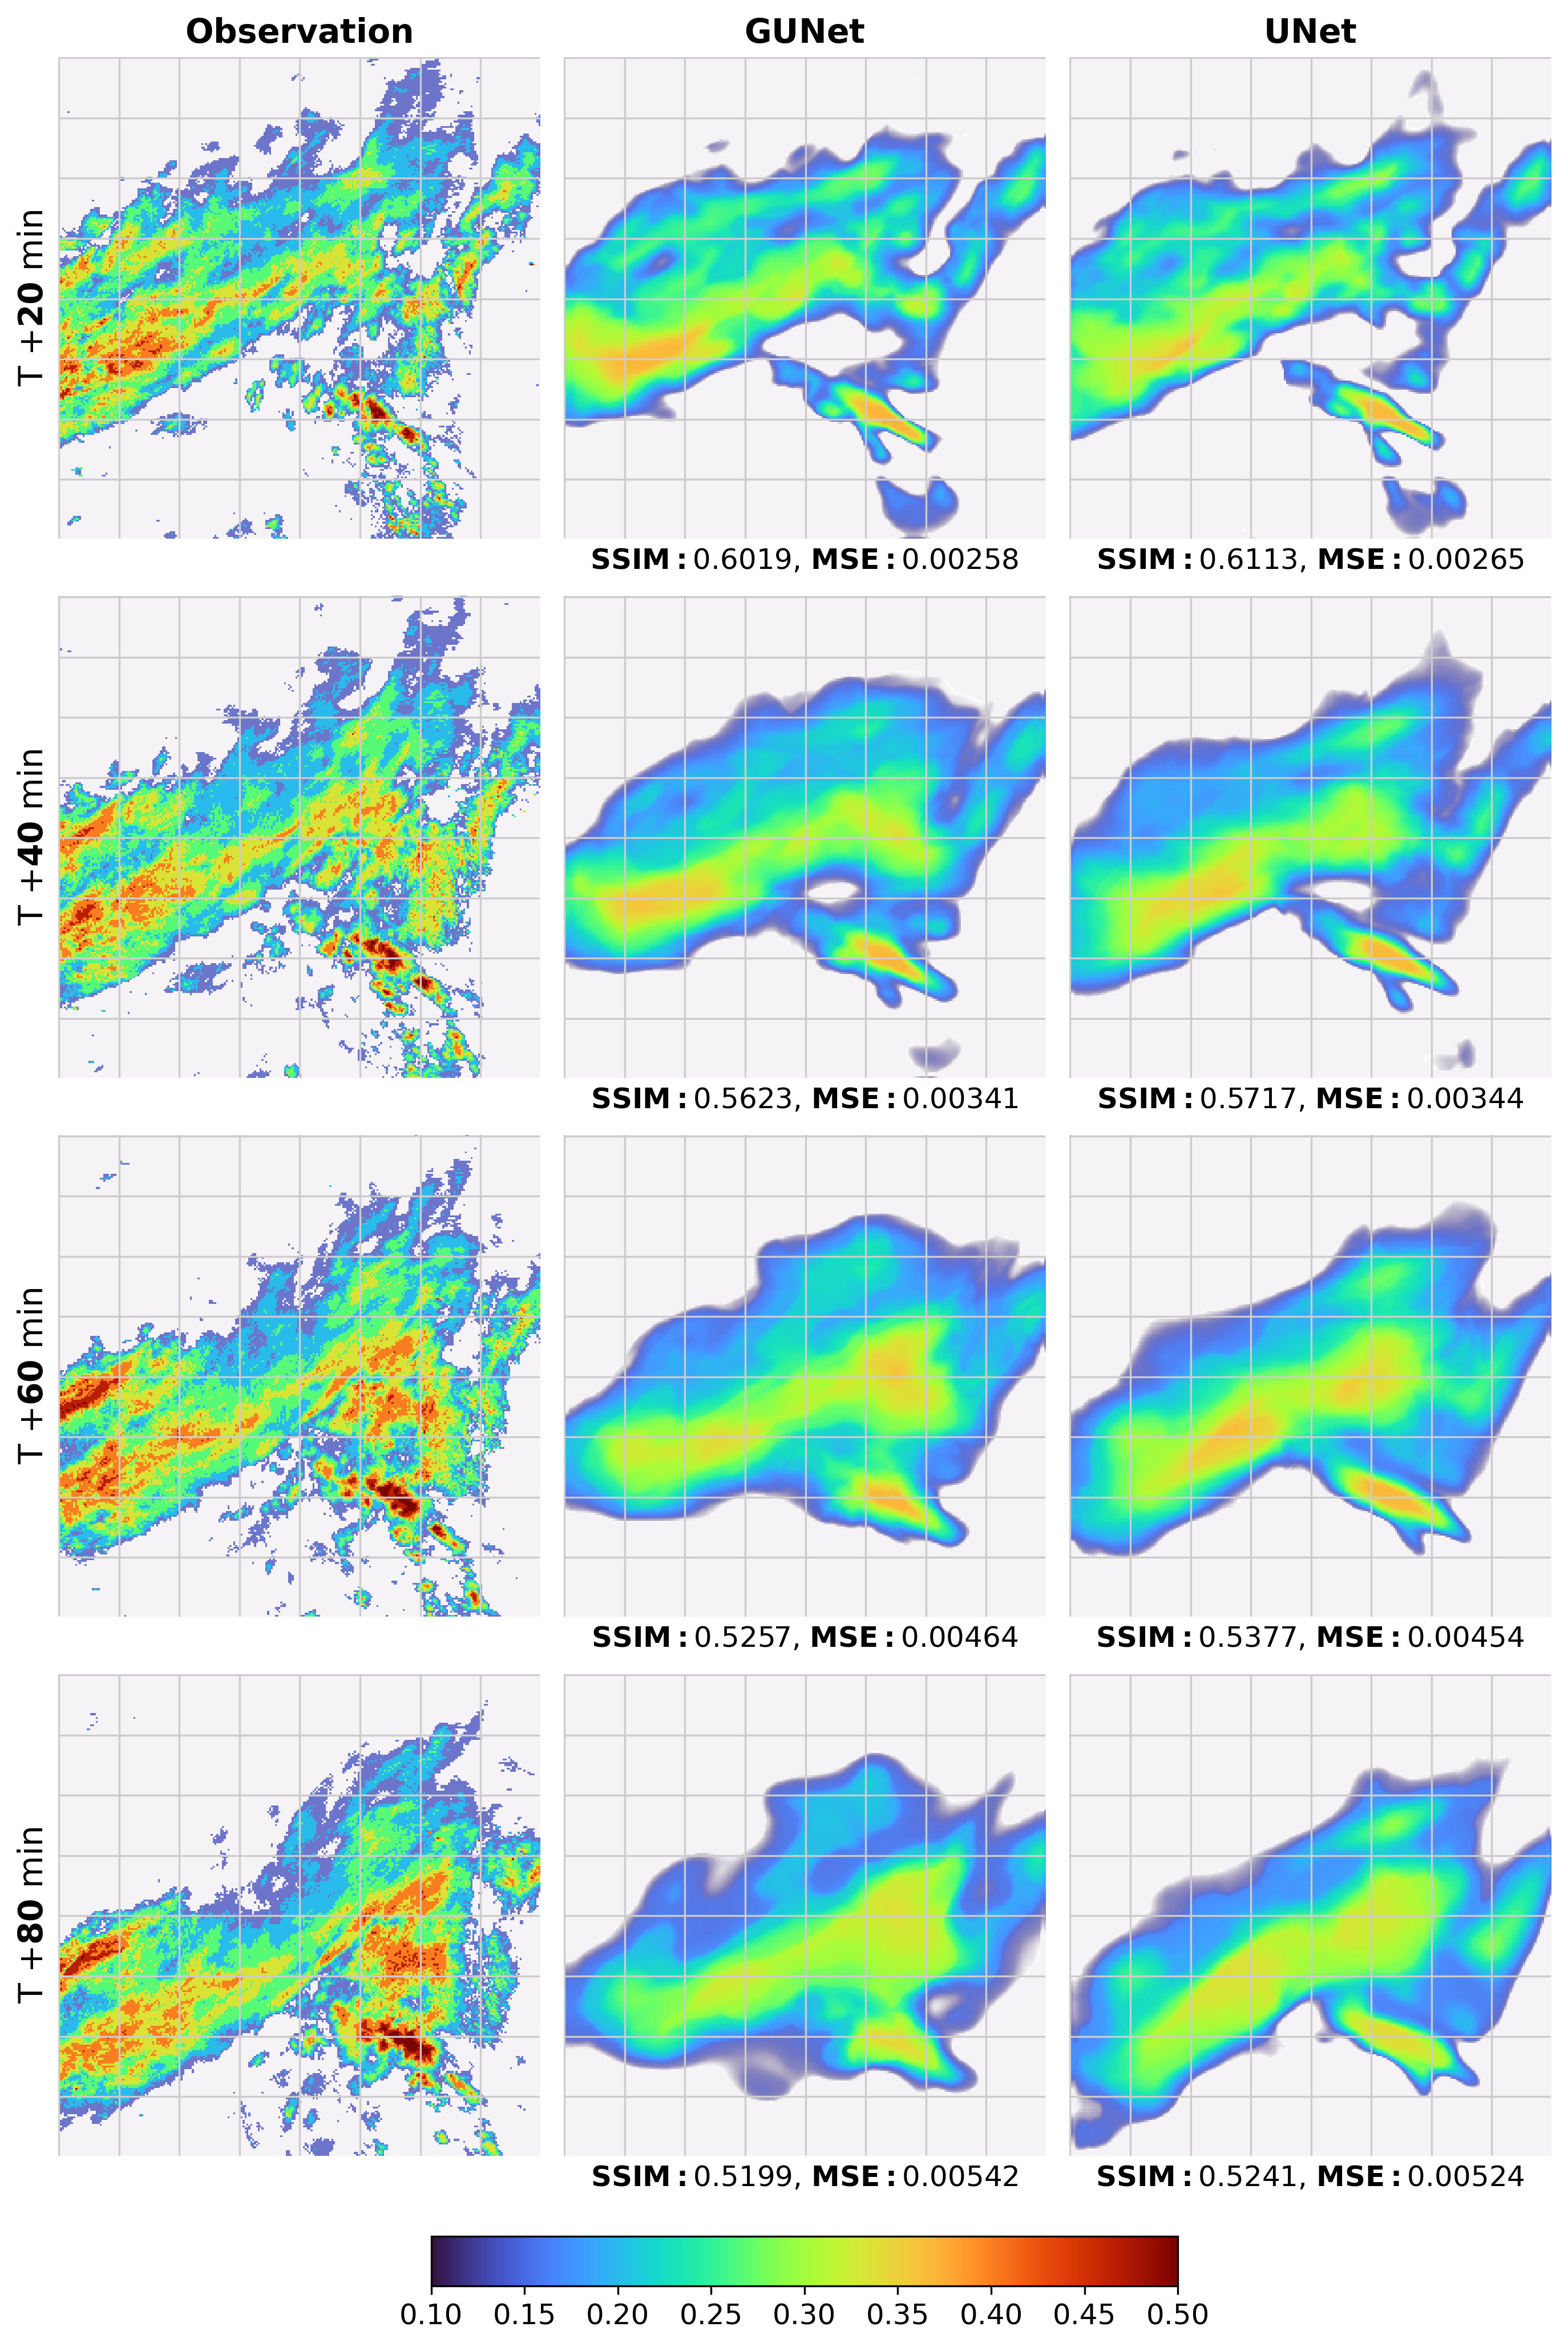
\includegraphics[width=\textwidth]{images/comparison_square_06.png}
    \caption[Comparison of weather predictions of both models (1)]{\label{fig:comparison_06}Comparison of UNet and GUnet outputs with ground truth observations.}
\end{figure}

\subsection{Forecast of Higher Intensity Storms}
\label{sec:forecast_higher_intensity}

To evaluate the performance of the models on higher-intensity storms, I set the values in the output and target tensors to 0 if they were below some threshold. I measured the metrics \gls{SSIM}, \gls{MAE}, and \gls{MSE} for different threshold values on the test dataset, the same way as I mentioned at the beginning of the chapter. Figure \ref{fig:threshold_ssim} shows that \gls{GUNet} achieved better performance than the UNet when $\texttt{threshold} \geq 0.2$.

As the threshold increases, fewer pixels are available for model comparison, leading to a decrease in performance differences between the models. At a $\texttt{threshold} \approx 0.35$, both models achieved the same level of performance in all metrics. Therefore, the discrepancy observed at $\texttt{threshold} = 0.2$ is unrelated to the natural decrease of the differences. If the threshold is high enough, both models can achieve an MSE and MAE of 0 and an SSIM of 1. The appendix includes figures \ref{fig:threshold_mae} and \ref{fig:threshold_mse}, demonstrating the relationship between threshold and \gls{MAE} and \gls{MSE}.


\begin{figure}[ht]
    \centering
    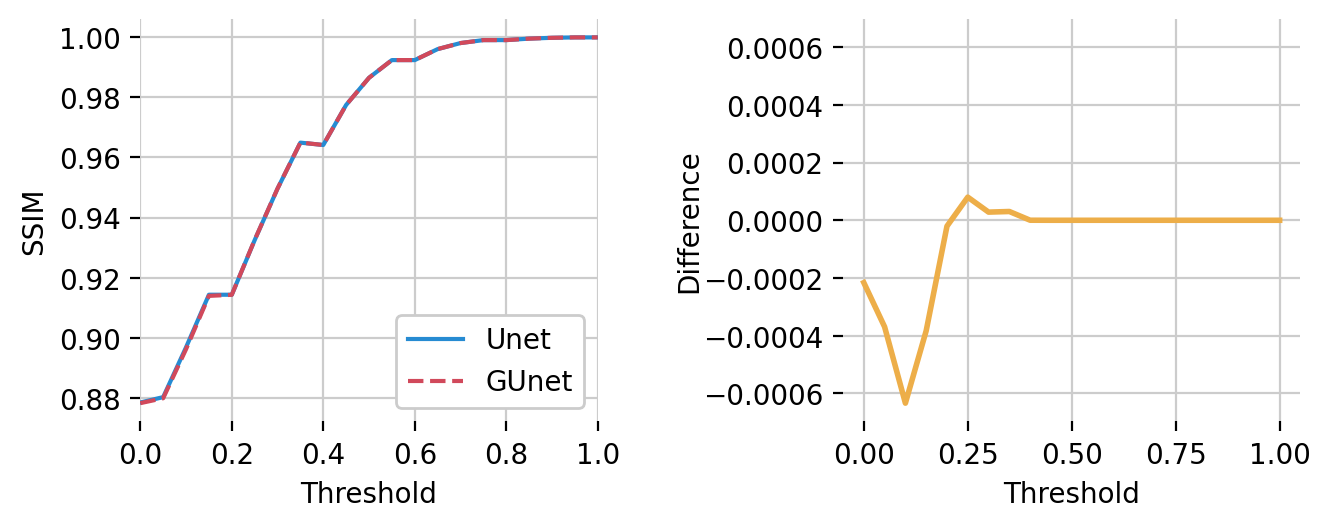
\includegraphics[width=\textwidth]{images/threshold_ssim.png}
    \caption[Higher intensity storm prediction metrics]{\label{fig:threshold_ssim}The test dataset was used to calculate the average \gls{SSIM}, comparing outputs and targets. Any values below a specified threshold were considered to be 0. The chart on the right displays the difference between $\texttt{ssim\_gunet} - \texttt{ssim\_unet}$ based on the threshold value.  Negative values indicate that UNet performed better in \gls{SSIM}, and positive values indicate that \gls{GUNet} had better \gls{SSIM}.}
\end{figure}

\section{Impact of Guided Upsampling on Spectral Bias}
\label{sec:impact_guided_upsampling}

In order to determine whether the \gls{GU} had any influence on the spectral bias by eliminating the structural bias\footnote{Reasoning behind this hypothesis was explained in section \ref{sec:bias}}, I followed a similar method to the one in the paper \cite{gunet}. I compared the average Fourier spectra of the targets and both models. I did this by averaging all outputs over the whole test dataset and computing a spectrum of the average using a 2D Fourier transform, equivalent to computing the Fourier spectra for each image and averaging that\footnote{The reason behind it is the linearity of the Fourier transform}. Let $\mathcal{D} = \{d_1, d_2, \dots, d_N\}$ be the set of data points, where each $d_i = \{I_{i1}, I_{i2}, \dots, I_{i8}\}$ represents a set of 8 images. I defined the function $\texttt{AvgMagSpectrum}$ to compute the magnitude spectrum of the average images across all data points and within each data point:

\begin{equation}
    \texttt{AvgMagSpectrum}(\mathcal{D}) = \left| \mathcal{F} \left( \frac{1}{8N} \sum_{i=1}^{N} \sum_{j=1}^{8} I_{ij} \right) \right|,
\end{equation}

\noindent where $\mathcal{F}\{\cdot\}$ denotes the Fourier Transform, and $|\cdot|$ represents the magnitude of the complex Fourier coefficients.

The function can be applied to the sets $\mathcal{D}_{\texttt{GUNet}}$, $\mathcal{D}_{\texttt{UNet}}$, and $\mathcal{D}_{\texttt{tgt}}$ to compute the magnitude spectra $\bar{M}_{\texttt{GUNet}}$, $\bar{M}_{\texttt{UNet}}$, and $\bar{M}_{\texttt{tgt}}$ for the respective \gls{GUNet} outputs, UNet outputs, and targets. After computing the magnitude spectra, the zero-frequency component was shifted to the center of the spectrum for better visualization and analysis. $\bar{M}_{\texttt{GUNet}}$, $\bar{M}_{\texttt{UNet}}$, and $\bar{M}_{\texttt{tgt}}$ are displayed in figure \ref{fig:fourier}.

\begin{figure}[ht]
    \centering
    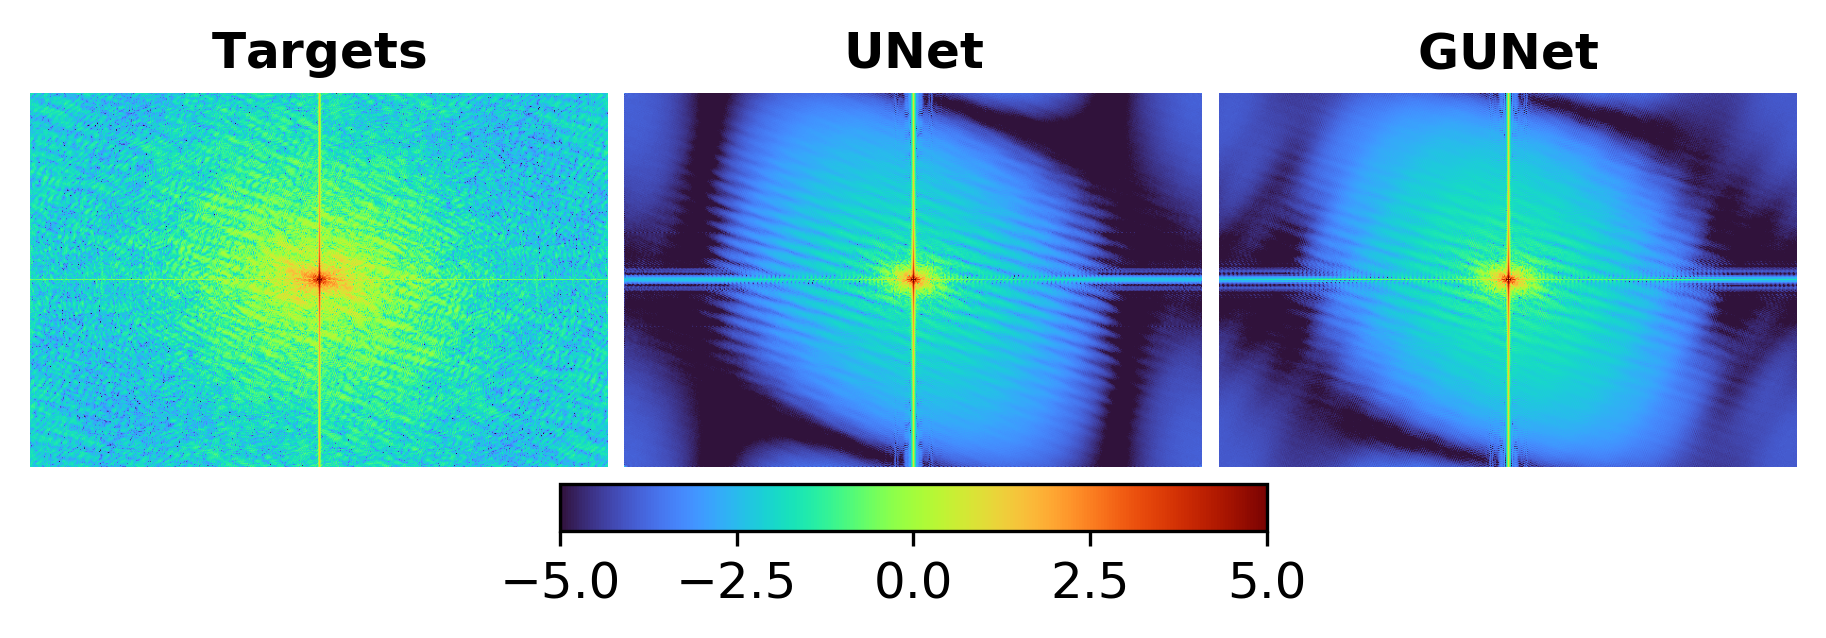
\includegraphics[width=\textwidth]{images/fourier.png}
    \caption[Comparison of average fourier spectra]{\label{fig:fourier}Average magnitude spectrum of UNet outputs $\bar{M}_{\texttt{UNet}}$, GUnet outputs $\bar{M}_{\texttt{GUNet}}$ and ground truth $\bar{M}_{\texttt{tgt}}$ on a logarithmic scale.}
\end{figure}

At first glance, the differences may not be immediately apparent. \gls{GUNet} seems to capture more of the higher frequencies\footnote{Higher frequencies are the ones further away from the center.}. To investigate this more thoroughly, I calculated the absolute value of the difference between the average spectrum of the targets and the average spectrum of the network outputs by computing:

\begin{equation}
    \texttt{diff}\left(\bar{M}_{m}\right)=\left| \bar{M}_{\texttt{tgt}} - \bar{M}_{m} \right|,
\end{equation}

\noindent where $\bar{M}_{m}$ is $\bar{M}_{\texttt{UNet}}$ or $\bar{M}_{\texttt{GUNet}}$. The result of this can be seen in figure \ref{fig:fourier_diff_1}. In the appendix  \ref{apx:comparisons}, I included figure \ref{fig:fourier_diff_2}, which shows a different plot of the same data, and figure \ref{fig:fourier_diff_3} that shows the difference between the output spectra of both models. Values were passed through moving average with a window size of 32×32, so the differences between the two spectra can be seen more clearly.

\begin{figure}[ht]
    \centering
    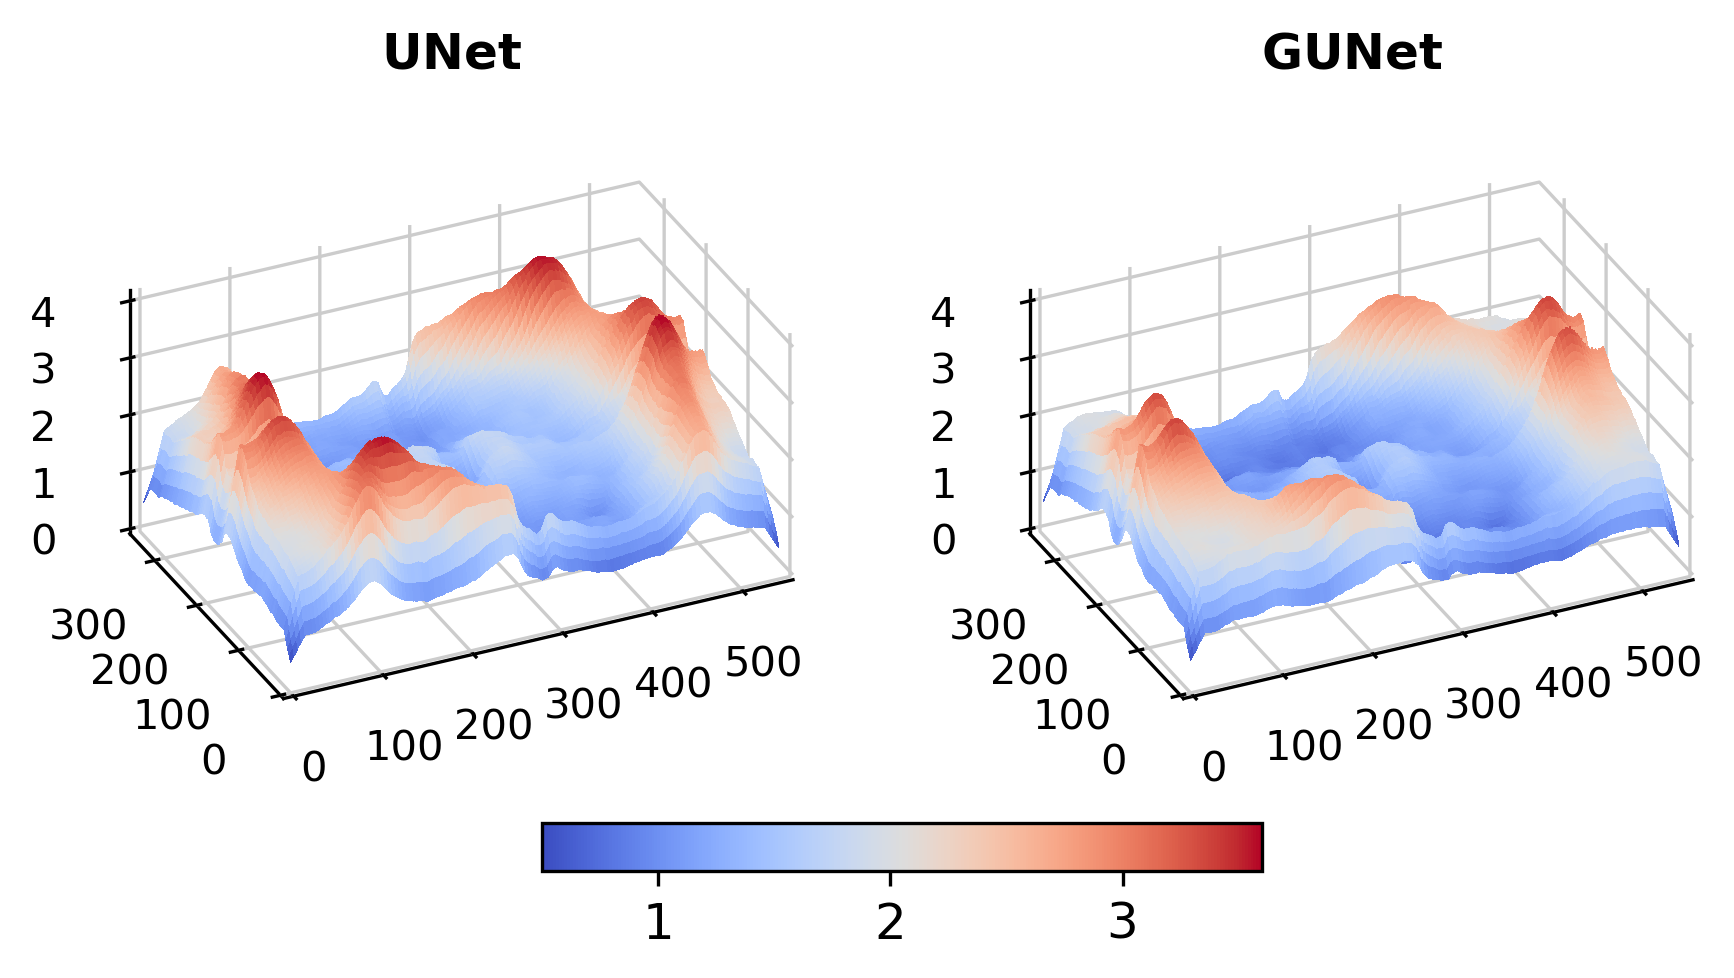
\includegraphics[width=\textwidth]{images/fourier_diff_1.png}
    \caption[Difference between the target and output spectra (3D plot)]{\label{fig:fourier_diff_1}Absolute difference between the amplitudes of the average target spectrum and the average output spectra of models on a logarithmic scale. Values were smoothed by moving average with kernel size 32×32. An unsmoothed 2D chart is in figure \ref{fig:fourier_diff_2}. A higher pixel value means that the amplitude, at the frequency corresponding to that pixel, differed more from the desired amplitude of the average target spectrum.}
\end{figure}

